\documentclass[border=6pt]{standalone}
\usepackage{tikz}
\usetikzlibrary{arrows.meta,positioning,calc,shapes.geometric,fit,backgrounds,patterns,matrix,decorations.pathreplacing}
\begin{document}
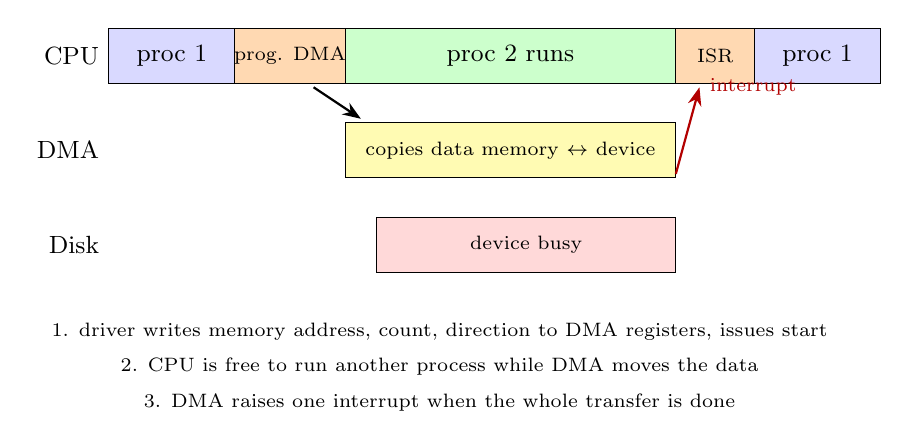
\begin{tikzpicture}[>=Stealth,font=\small]
\tikzstyle{lane}=[draw,minimum width=9.5cm,minimum height=0.7cm,anchor=west]
\node[anchor=east] at (0,2.4) {CPU};
\node[anchor=east] at (0,1.2) {DMA};
\node[anchor=east] at (0,0) {Disk};
\draw[fill=blue!15] (0,2.05) rectangle node{proc 1} (1.6,2.75);
\draw[fill=orange!30] (1.6,2.05) rectangle node{\scriptsize prog. DMA} (3,2.75);
\draw[fill=green!20] (3,2.05) rectangle node{proc 2 runs} (7.2,2.75);
\draw[fill=orange!30] (7.2,2.05) rectangle node{\scriptsize ISR} (8.2,2.75);
\draw[fill=blue!15] (8.2,2.05) rectangle node{proc 1} (9.8,2.75);
\draw[fill=yellow!30] (3,0.85) rectangle node{\scriptsize copies data memory $\leftrightarrow$ device} (7.2,1.55);
\draw[fill=red!15] (3.4,-0.35) rectangle node{\scriptsize device busy} (7.2,0.35);
\draw[->,thick] (2.6,2.0) -- (3.2,1.6);
\draw[->,thick,red!70!black] (7.2,0.9) -- (7.5,2.0) node[right,font=\scriptsize]{interrupt};
\node[font=\scriptsize,align=left] at (4.2,-1.1) {1. driver writes memory address, count, direction to DMA registers, issues start};
\node[font=\scriptsize,align=left] at (4.2,-1.55) {2. CPU is free to run another process while DMA moves the data};
\node[font=\scriptsize,align=left] at (4.2,-2.0) {3. DMA raises one interrupt when the whole transfer is done};
\end{tikzpicture}
\end{document}
